\subsection{Observation af fodgængerfeltet}
\label{sub:foerste_obs}
Da størstedelen af cyklisterne ud fra trafiktællingerne færder sig omkring fodgængerfeltet, blev der observeret her første gang med det formål, at se om der var nogle konflikter, der kunne undersøges videre.
Aalborg er byen som arbejder på, at skabe en cykelby.\autocite{aabcykelby}
Som en cykelby kræver det, at der er en optimal sikkerhed for cyklister blandt andre trafikantgrupper. Trafik flowet ved åbningen af Nytorv blev observeret, området ved McDonalds og Burger King, hvor der kunne ses, at de fleste cyklister havde nogle mindre alvorlige konflikter med bilerne, som krydser Nytorv illegalt. Tværtimod havde cyklisterne lidt større konflikter med fodgængere, hvilket også gav et stop for trafik flowet. Derudover kunne der ikke observeres en tryghed på cyklisterne, eftersom de hele tiden skulle være fokuseret og parat til, at bremse ned for fodgængere eller busser. En mindre vurdering kunne bekræfte, at fodgængerne ikke havde en optimal tryghed ved området på grund af cyklisterne.
Eftersom cyklisterne var et problem for fodgængerne, så blev cyklisterne observeret grundigere. Der blev også identificeret, at fodgængere var delvis utryg ved Nytorv området, hvilket gav årsag til grundigere undersøgelse, såsom interview med fodgængere.

\subsection{Dybere undersøgelse for observationen af fodgængerfeltet}
\label{sub:dyb_undersoelse}
I første omgang blev der blot observeret, hvor der blev antaget en række antagelser, hvoraf der til næste observation blev gjort brug af mere specifikke metoder for at identificere sikkerheden ved Nytorv området i Aalborg.
%\\\\
Metoderne bag næste observation var at identificere konflikter ved området. Ved hjælp af konflikterne kan sikkerheden for de forskellige trafikantgrupper identificeres. Inden metoderne bliver præsenteret, vil begrebet konflikt blive defineret først. Begrebet konflikt er et meget vidt begreb og dækker indenfor flere fagområder, men i denne rapport bliver begrebet nærmere undersøgt indenfor vej og trafik. Som umiddelbart vil man definere en konflikt, som værende sammenstød mellem to trafikkanter, men dog udelukker den svenske trafikteknik denne påstand. \autocite{sweconflict}
En af metoderne, som bliver anvendt til identificering af konflikterne, er den svenske traftikteknik, hvilket er årsagen til deres definition af konflikt bliver brugt i dette projekt.
%\\\\
Den svenske trafikteknik beskriver en konflikt mellem to trafikkanter, som har kollisionskurs og vil kolligere, hvis en af trafikkanterne ikke foretager sig en pludselig afværgning.2 Det vil sige, at så længe et uheld (sammenstød) kan undgås af mindst en af trafikanterne, så vil der stadig være tale om en konflikt \autocite{sweconflict}. Ved hjælp af den svenske trafikteknik, kan man dele en konflikt i flere grader. De forskellige konfliktgrader er defineret som alvorlige konflikter, mindre alvorlige konflikter og potentielle konflikter, som også kan ses på \cref{fig:indellingkonflikter} side \pageref{fig:indellingkonflikter}:
 \begin{figure}[htbp]
   \centering
   \begin{adjustbox}{max width=\textwidth}
     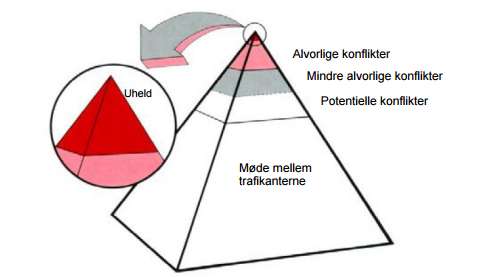
\includegraphics{figures/Billederogfigur/konflikt.png} %http://www.trafitec.dk/sites/default/files/publications/konfliktteknikstudier%20i%20kbh%20bykryds.pdf
  \end{adjustbox}
   \caption{Inddeling af konflikter \autocite{konfli}}
    \label{fig:indellingkonflikter}
 \end{figure}
 \newpage


 En konfliktgrad bestemmes ved hjælp af en TA-værdi. TA-værdien er defineret som tid til ulykke, altså Time to Accident. Metoden bag bestemmelse af TA-værdien gøres ved hjælp af følgende formel:

 $$TA=\frac{d}{V} $$ \autocite{konfli}

Hvoraf $$TA beskriver tid til ulykke$$ \\ $$d, beskriver distancen til tænkt kollisionspunkt$$ \\ og $$V, er hastigheden i den undvigeøjeblik.$$

Formlen fortæller om forholdet mellem distancen til det potentielle punkt i en kollision og hastigheden, når en af trafikanterne undviger uheldet. Heraf kan der ved hjælp af \cref{fig:tagraff} side \pageref{fig:tagraff},
ses om konflikten er alvorlig eller ej.
%~\\\\

\begin{figure}[htbp]

  \centering
  \begin{adjustbox}{max width=\textwidth}
    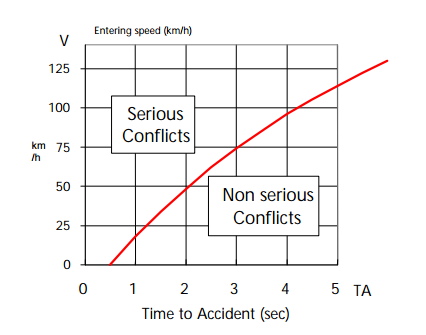
\includegraphics{figures/Billederogfigur/tugraf.png} %http://www.tft.lth.se/fileadmin/tft/video_in_traffic/Swedish_conflict_technique.pdf
 \end{adjustbox}
  \caption{TA-graf \autocite{sweconflict}}
    \label{fig:tagraff}
\end{figure}

Som der kan ses på \cref{fig:tagraff} side \pageref{fig:tagraff}
, så er alvorligheden af en konflikt afhængig af både distance samt hastighed.
Som udgangspunkt i TA-grafen kan der ses, at en TA-værdi over 0.5 ses som ikke alvorlig konflikt, hvorimod en TA-værdi under ca. 0.5, vil være en alvorlig konflikt.



For at kunne beregne TA-værdien, skal distancen og hastigheden kendes. Distancen og hastigheden kan identificeres ved blot nogle målinger ved området, hvilket i dette projekt blev gjort, som ses på figur \cref{fig:obsomrrod} side \pageref{fig:obsomrrod} og figur \cref{fig:obsomrbla} side \pageref{fig:obsomrbla}
%\\\\

Som der kan ses på figur \cref{fig:obsomrrod} side \pageref{fig:obsomrrod} og figur \cref{fig:obsomrbla} side \pageref{fig:obsomrbla}
blev området i første omgang målt op fra kanten, som er markeret med farven rød, til fodgængerfeltet og ligeså fra den anden kant, som er markeret med farven blåt. Bemærk de andre markeringer på figuren, som bruges til beregning af TA-værdien, er forskellige længder, altså er d forskellig i formlen for TA-værdien : $$ TU=\frac{d}{V} $$

\begin{figure}[htbp]
   \centering
   \begin{adjustbox}{max width=\textwidth}
     \includegraphics[scale=0.3]{figures/billederogfigur/rodmarkering.jpg}
  \end{adjustbox}
   \caption{Måling fra den højre kant}
   \label{fig:obsomrrod}
 \end{figure}

 \begin{figure}[htbp]
    \centering
    \begin{adjustbox}{max width=\textwidth}
      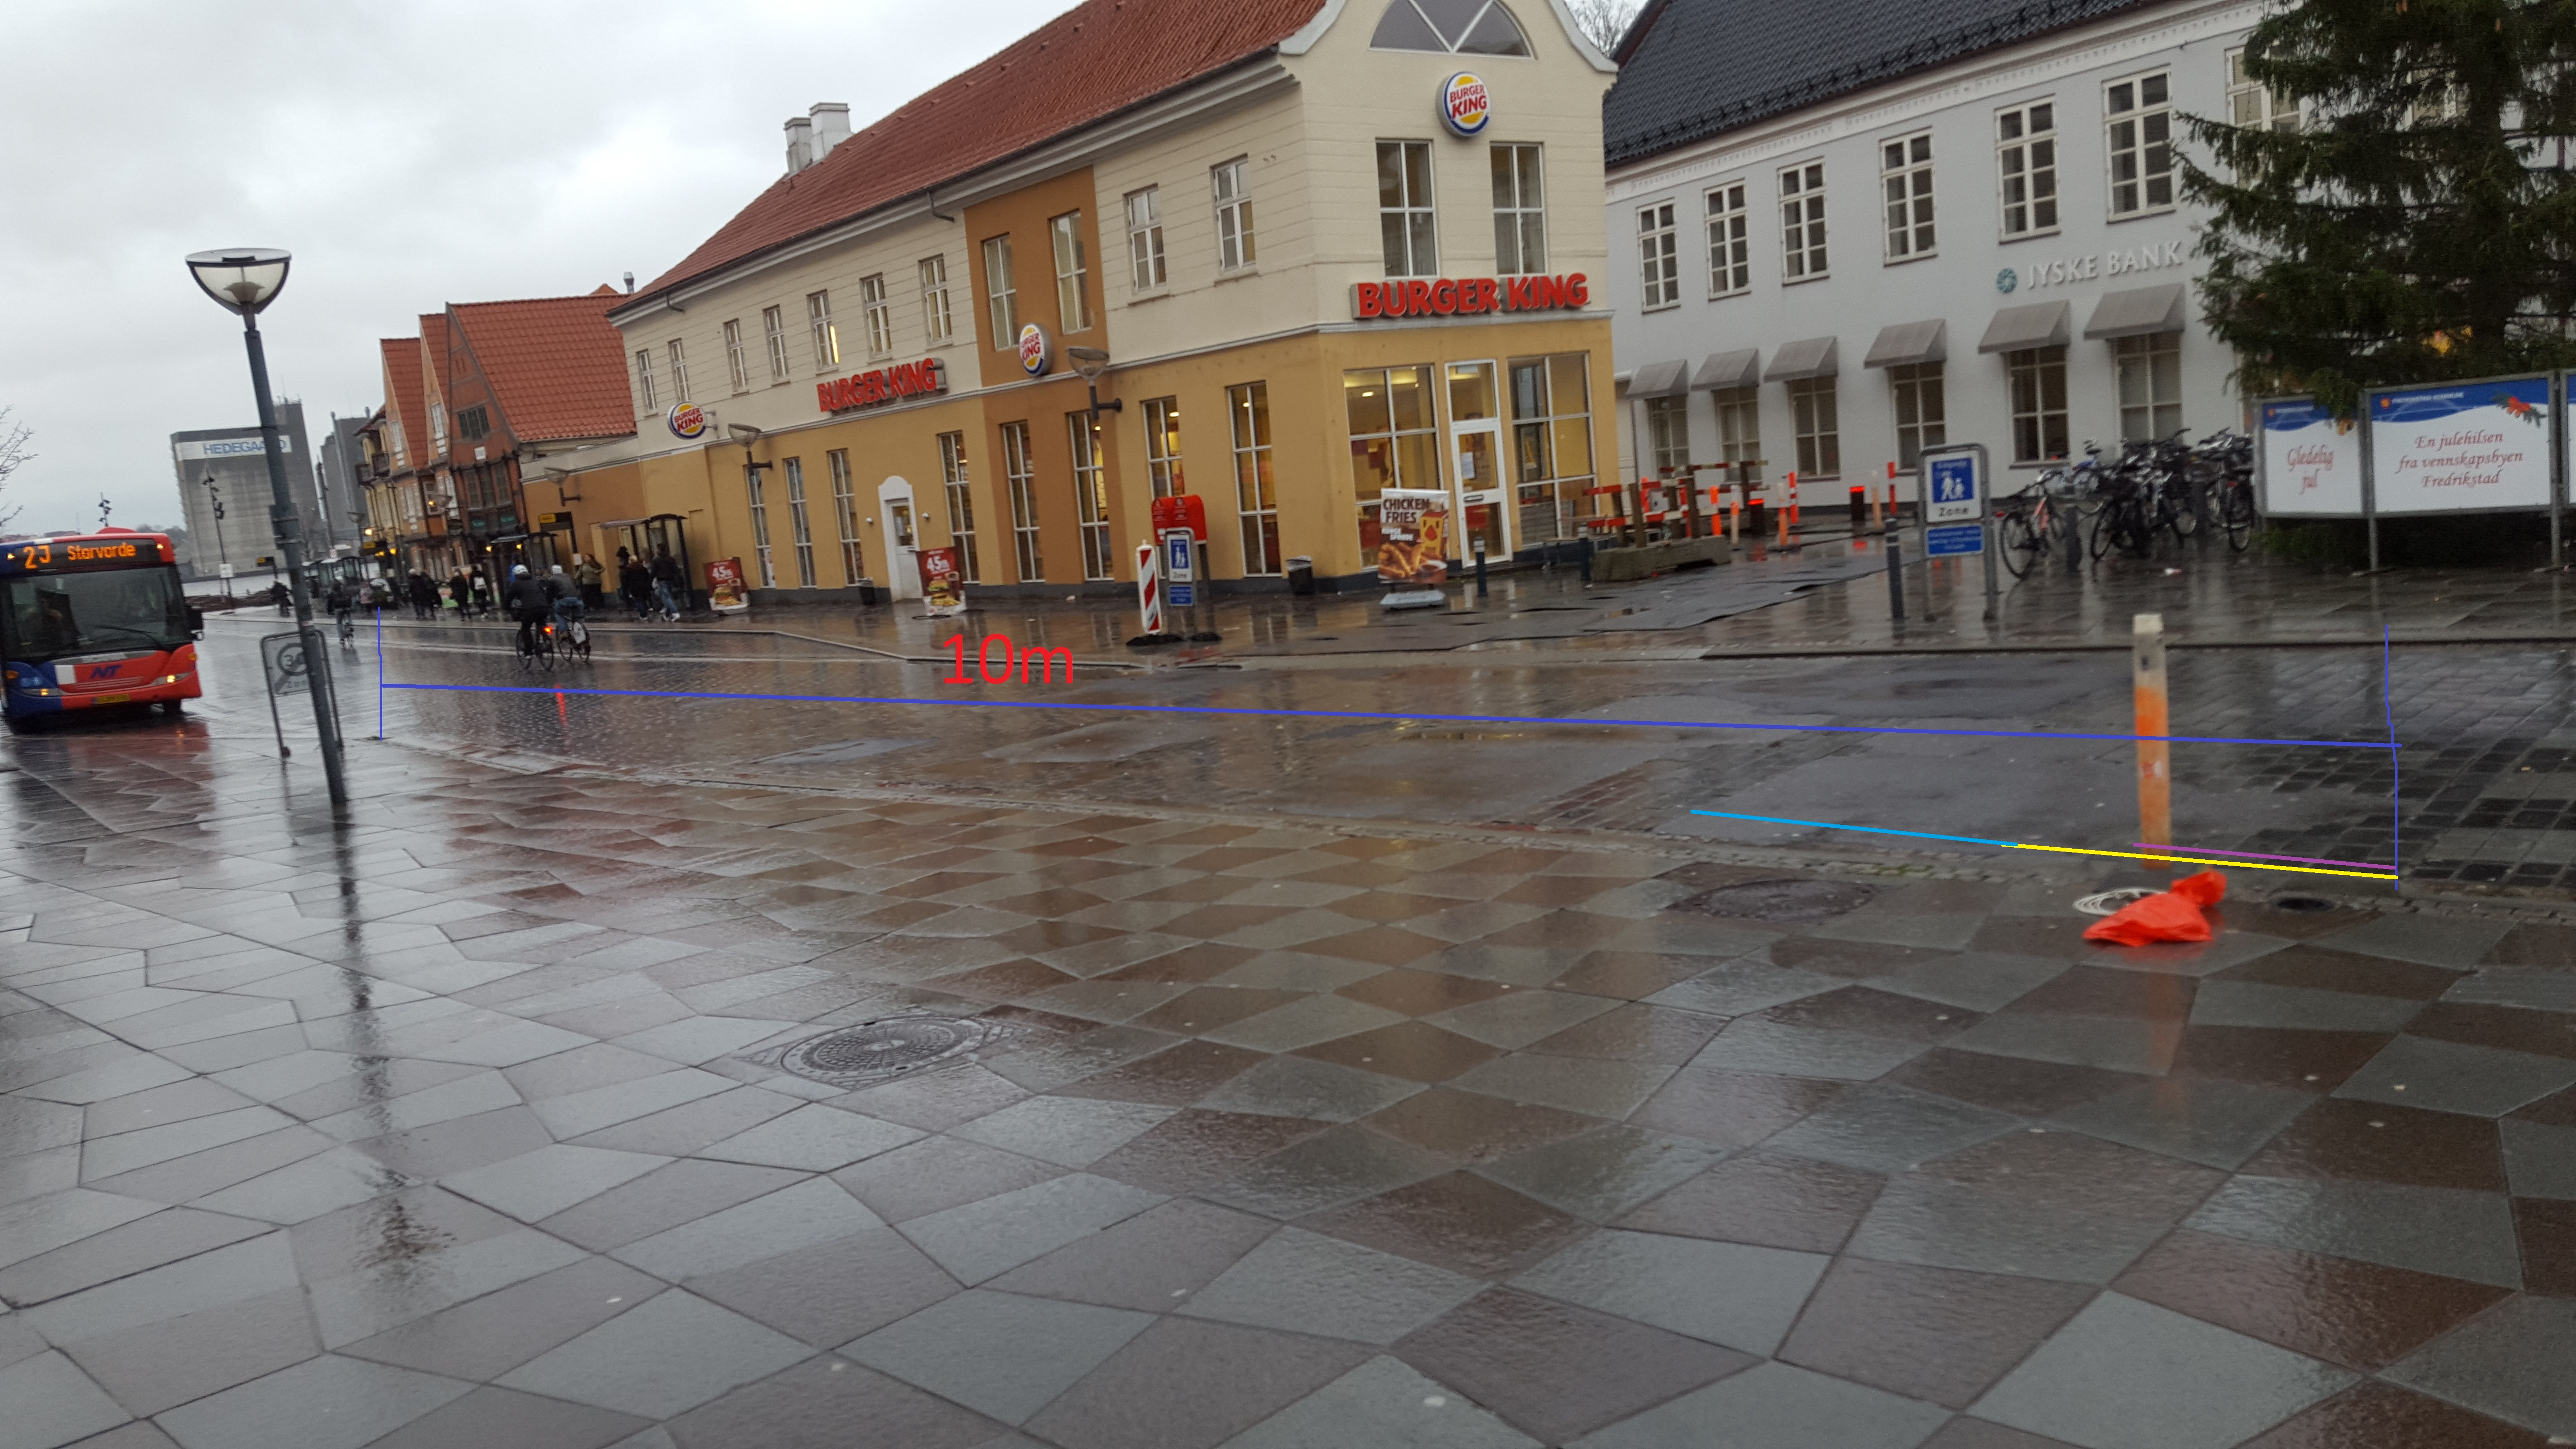
\includegraphics[scale=0.3]{figures/billederogfigur/blaamarkering.jpg}
   \end{adjustbox}
    \caption{Måling fra den venste kant}
    \label{fig:obsomrbla}
  \end{figure}


%\begin{figure}
%\centering
%\begin{subfigure}{1\textwidth}
 % \centering
  %\includegraphics[width=1\linewidth]{figures/billederogfigur/rodmarkering.jpg}
  %\caption{A: Måling fra den højre kant}
  %\label{fig:obsomrrod}
%\end{subfigure}
%\begin{subfigure}{2\textwidth}
 % \centering
  %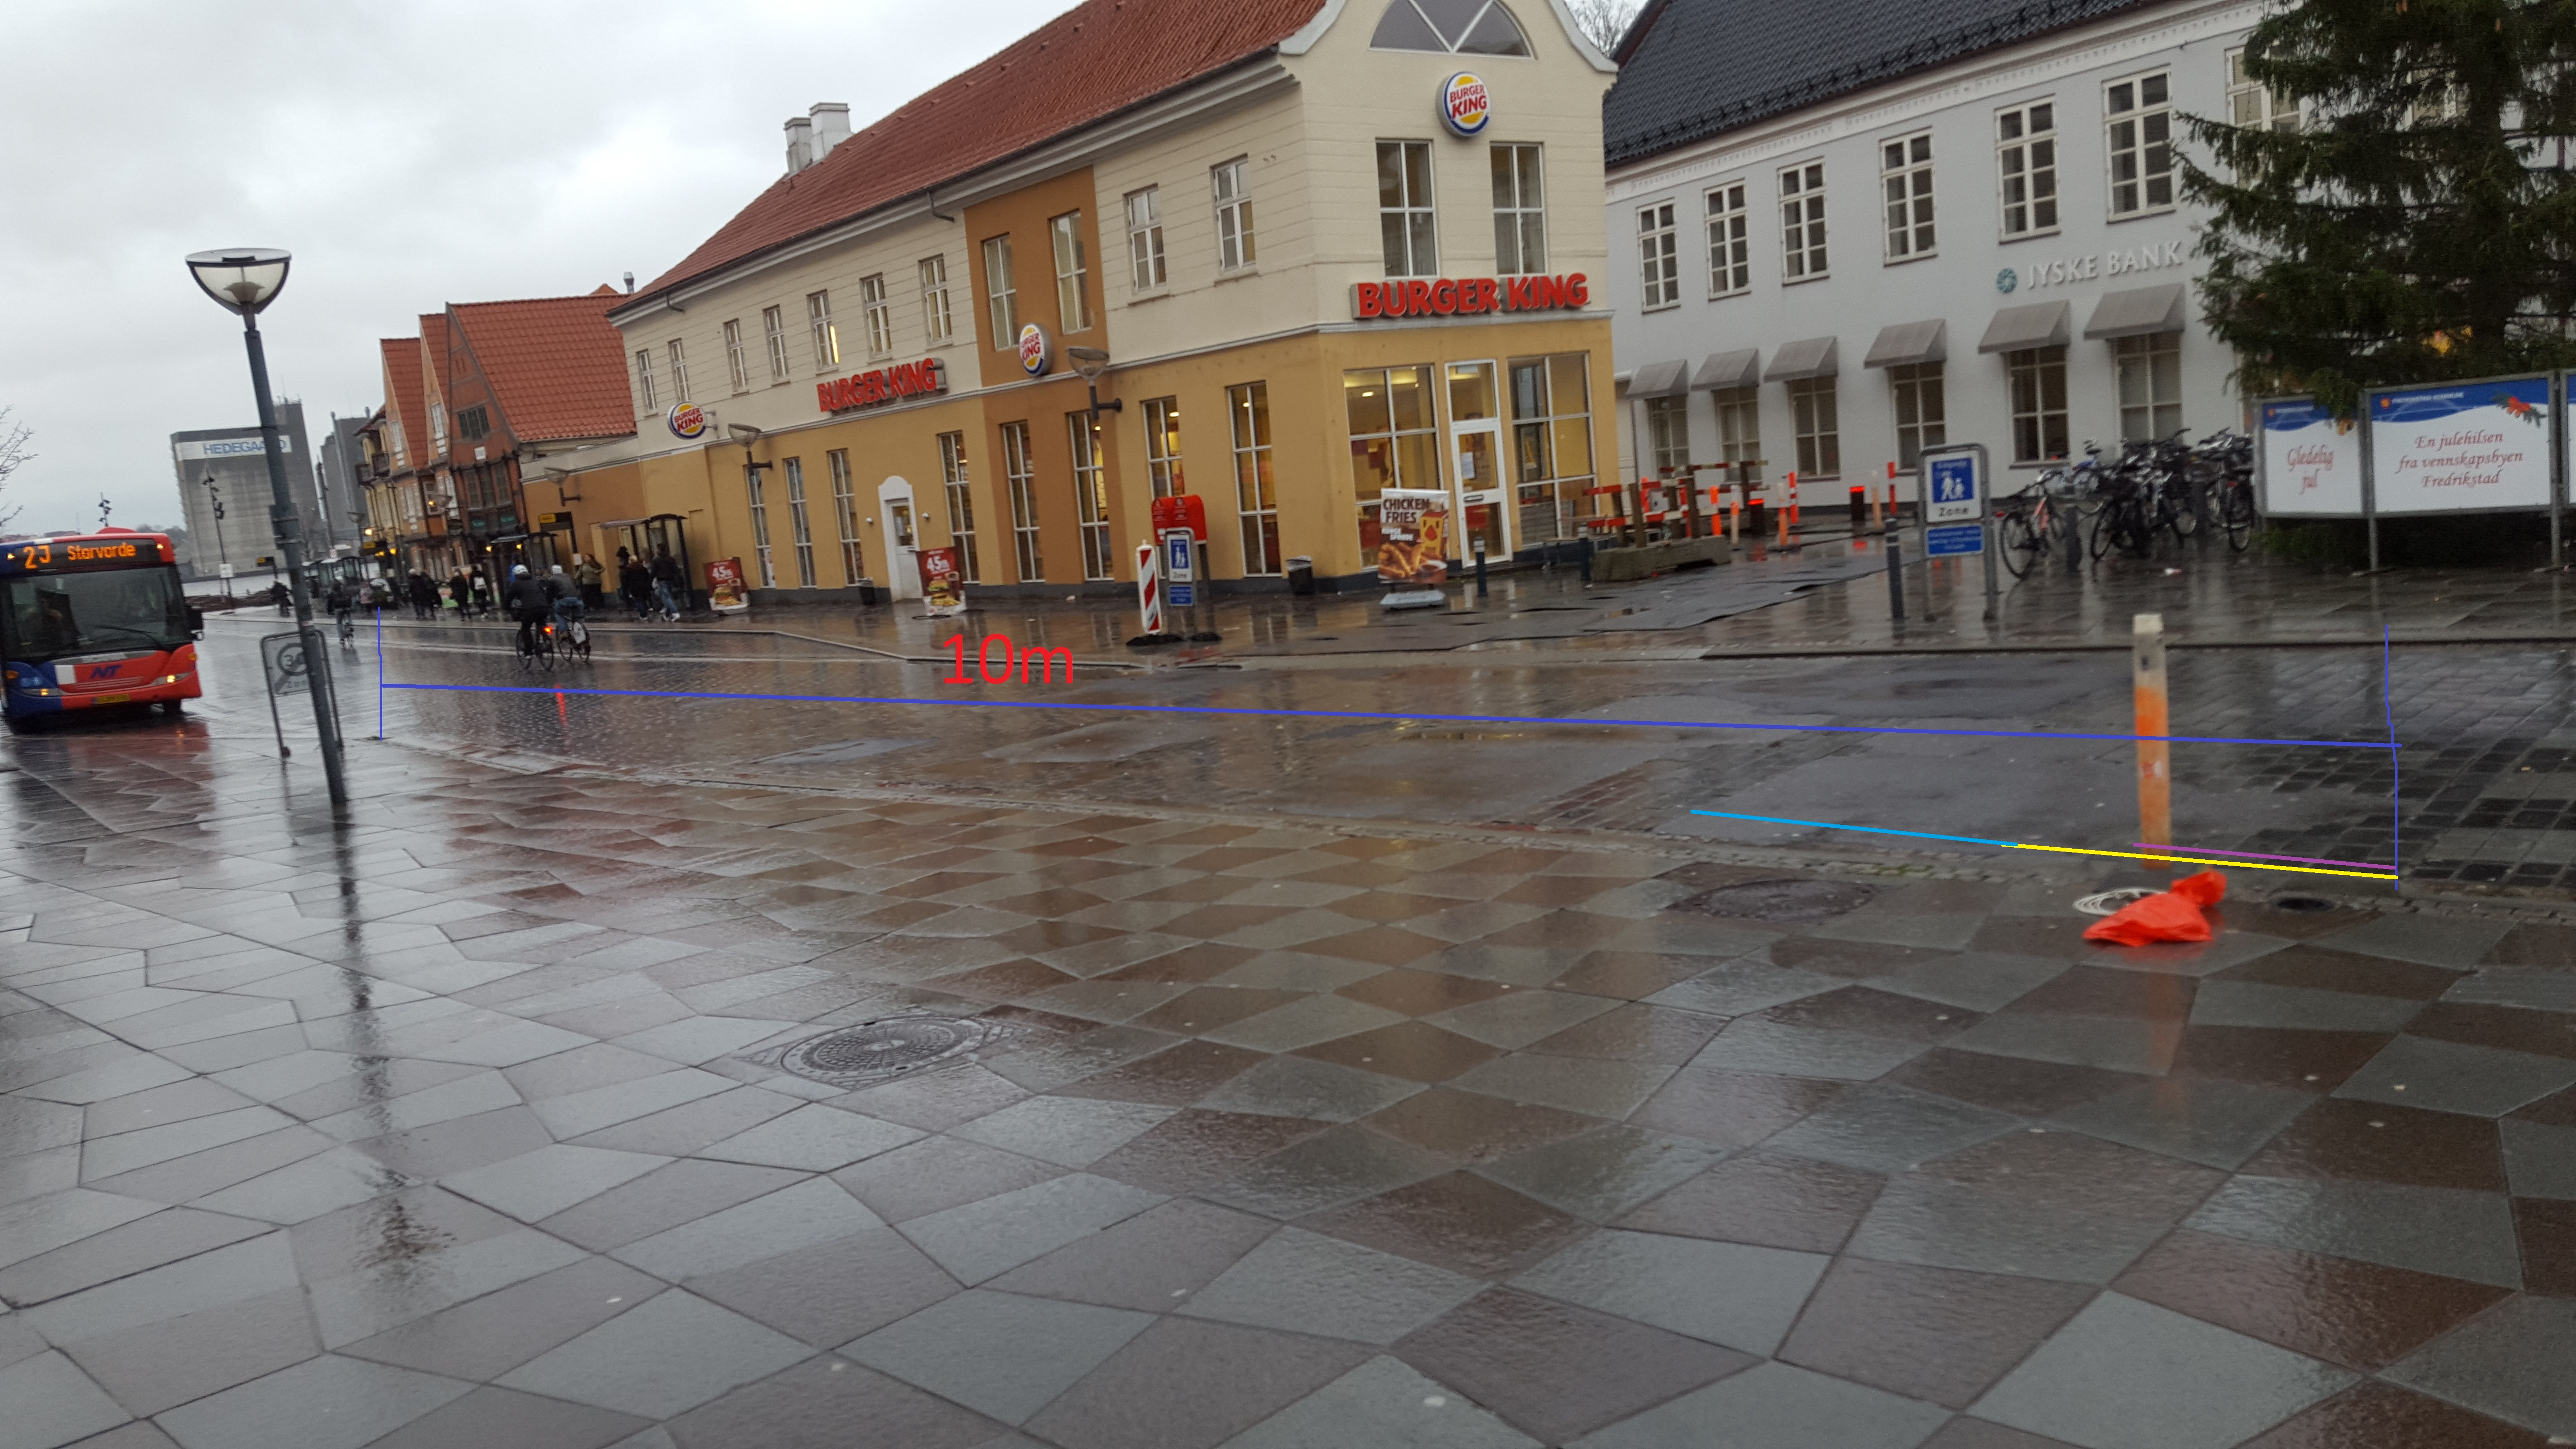
\includegraphics[width=1\linewidth]{figures/billederogfigur/blaamarkering.jpg}
  %\caption{B: Måling fra den venstre kant}
  %\label{fig:obsomrblaa}
%\end{subfigure}
%\caption{Målinger fra begge sider}
%\label{fig:maalingerfrabegge}
%\end{figure}
Herefter var metoden bag TA-værdien, at der blev lavet nogle målinger. De forskellige distancer blev noteret, og derudover blev der også taget tid til hver enkelt konflikt.~\\

Starttidspunkt: 13:00
~\\
Sluttidspunkt:15:00
~\\
Placering: Fodgængerfeltet ved Bispengade
~\\
Observationssted: Guiness Bar udenfor
~\\
Anvendt materiale: Computer og tidsfornemmelse, stopur
~\\
Fejlkilder: Regnvejrsdag, egen tidsfornemmelse
~\\
Afstand fra havn til fodgængerfelt, som blev brugt til at måle hastighed: 10m
~\\
Afstand fra Jyske bank til fodgængerfelt: 10m
~\\\\
I første omgang blev tiderne af TA-værdi antaget, som vises i tabellen Antaget TA-værdier
\\\\
\begin{tabular}{ |p{1cm}|p{4cm}|p{4cm}|p{4cm}|  }
\hline
\multicolumn{3}{|c|}{Antaget TA-værdier} \\
\hline
Cykel & Hastighed [km/t] & TA-værdi [s]  \\
\hline
1 & 6   & 1.5  \\
2 & 10  & 0.7  \\
3 & 4.6 & 1.5  \\
4 & 11  & 0.4  \\
5 & 10  & 1  \\
6 & 9   & 0.1 \\
7 & 12  & 0.6  \\
8 & 10  & 0.7  \\
9 & 14  & 0.4  \\
10 & 8  & 1  \\
11 & 12 & 0.3  \\
12 & 11 & 0.6 \\
13 & 10 & 0.8 \\
14 & 6  & 1 \\
15 & 9  & 0.9 \\
16 & 10 & 0.5 \\
17 & 14 & 0.3 \\
18 & 12 & 0.6 \\
19 & 7  & 1 \\
20 & 5  & 1.5 \\
\hline
%\caption{Antaget TA-værider}
%\label{tab:antaget_tavardi}
\end{tabular}



\subsection{Resultater af observation}
\label{sub:def_konflikt}
Som tidligere nævnt, så blev distancen for hvert konflikt noteret, hvilket gør det muligt, at beregne en mere præcis TA-værdi. Tabel %-cref{tab:beregnede_tavardi},
viser den beregnede TA-værdi for den bestemte hastighed samt distance, som blev målt under udførelsen af metoden.
\\
\begin{tabular}{ |p{1cm}|p{4cm}|p{4cm}|p{4cm}|  }
\hline
\multicolumn{4}{|c|}{Beregnet TA-værdier} \\
\hline
Cykel & Hastighed [m/s] & TA-værdi [s] & Distance [m] \\
\hline
1 & 1.6   & 1.25 & 2 \\
2 & 2.8 & 0.1 & 0.5 \\
3 & 1.3 & 1.5 & 2 \\
4 & 3  & 0.3 & 1 \\
5 & 2.8  & 0.7 & 2 \\
6 & 2.5   & 0.2 & 0.5 \\
7 & 3.3  & 0.1 & 0.5 \\
8 & 2.8  & 0.3 & 1 \\
9 & 3.9  & 0.1 & 0.5\\
10 & 2.2  & 0.9   & 2 \\
11 & 3.3 & 0.3 &  1 \\
12 & 3.1 & 0.6 &   2\\
13 & 2.8 & 0.3 & 1\\
14 & 1.6  & 1.25   & 2\\
15 & 2.5  & 0.4 & 1\\
16 & 2.8 & 0.3 & 1\\
17 & 3.9 & 0.13 &0.5\\
18 & 3.3 & 0.1 & 0.5\\
19 & 1.9  & 1 & 2\\
20 & 1.4  & 1.4 & 2\\
\hline
%\caption{Beregnede TA-værider}
%\label{tab:beregnede_tavardi}
\end{tabular}
\\\\
%Som beskrevet i afsnit -cref{sub:def_konflikt}, så kan grafen for TA-værdien bruges til at identificere, hvor alvorlig konflikterne egentlig er ved området. I grafen kan der ses, hvor de beregnede TA-værdier er placeret, altså om de tilhører en alvorlig konflikt eller ej.
Som beskrevet i afsnit %-cref{sub:def_konflikt},
så kan grafen for TA-værdien bruges til at identificere, hvor alvorlig konflikterne egentlig er ved området. I grafen kan der ses, hvor de beregnede TA-værdier er placeret, altså om de tilhører en alvorlig konflikt eller ej.
%!!(GRAF skal laves, hvor der er en tildeling af konfliktgraderne, herunder skal beregnede TA-værdier sættes ind)!!
Som der kan ses på grafen, så er størstedelen af konflikterne ret alvorlige, eftersom trafikanterne kommer ret tætte på hinanden ved nogle bestemte hastigheder.
%\\\\
Mens den svenske trafikteknik blev udført ved området, blev der også udført adfærdsregistering ved området. Metoden bag adfærdsregistering vil blive introduceret inden udførselen bliver præsenteret.
Når	man	vil	observere nogle	konflikter mellem to eller flere	forskellige trafikantgrupper,	må man lave	nogle antagelser	om, hvad	 der egentlig vil føre til en konflikt. Man må altså	på	forhånd	opstille nogle hypoteser, som man via nogle undersøgelsesspørgsmål, kan bruge til	at forudse nogle	formåede	konflikter mellem nogle bestemte	trafikantgrupper.	Baggrunden for denne	måde at	undersøge konflikter	på ligger i,	at man sjældent 	vil	have	mulighed	 for at	observere selve konflikterne	eller uheldene, da det ikke	vil	være	 dagligdag på	 det	 givne observationssted.	I denne	undersøgelse om	fodgængernes sikkerhed på	Nytorv,	vil man altså ikke på observationsdagen formode,	at man direkte vil observere en alvorlig konflikt eller	et uheld mellem	en fodgænger og	en cyklist.	Måden man derimod	vil	kunne undersøge	de opstillede hypoteser på og bygge sine	spørgsmål op omkring, vil	være	at bruge en	evalueringsmetode, hvor	man	kigger på adfærdsstudier.i Her fokuserer	man	på den typiske normale adfærd på	sit observationssted, og	det skal så	underbygge	hypoteserne. Hele ideen bag denne evalueringsmetode er at ”forcere indhentningen af data”	(samme	kilde),	altså at forudsige data	som	belæg for sine antagelser.
I denne undersøgelse vil	adfærdsregistreringen blive bygget op omkring	figuren \cref{fig:adfreg} på side \pageref{fig:adfreg},
hvor fokus ligger på dels ankomsten mellem fodgængere	 og cyklister på observationsstedet. Udgangspunktet herfra er så at	undersøge, om	der i samtidige ankomster er et tidligt samspil eller	et sent samspil mellem de to trafikanter, hvilket er defineret ved hjælp af TA-værdier.
Herefter vurdere, om hændelse ud fra	de to parametre gik godt, om	der	opstod en konflikt	eller der decideret skete et	uheld. Hypotesen er	så,	at hvis	antallet af	tidlige samspil stiger og antallet af sene samspil falder, så vil trafiksikkerheden blive forøget.
\begin{figure}[htbp]
  \centering
  \begin{adjustbox}{max width=\textwidth}
    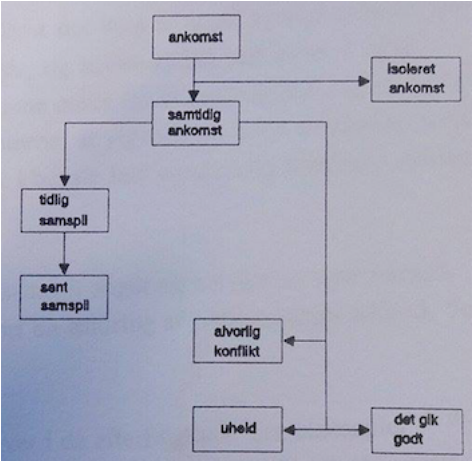
\includegraphics[scale=0.7]{figures/Billederogfigur/adfaerdsreg.png} %papir fra vejledern
 \end{adjustbox}
  \caption{Adfærdsregistrering}
    \label{fig:adfreg}
\end{figure}
~\\\\
\subsection{Adfærdsregistrering}
\label{sub:adfregis}
Dette afsnit er udarbejdet ud fra kilden: Konfliktteknik og adfærdsstudier.
%\\
For	at kunne registrere den typiske normale adfærd ud	 fra figuren, er det vigtigt at definere	de	forskellige	begreber. I tabel (??) kan man se en	opdeling af de forskellige begreber, en definition af dem og en optælling af de forskellige tilfælde. Alle	tilfældene finder sted i	en samtidig ankomst, da der i en isoleret ankomst	 ikke vil kunne	opstå en konflikt mellem to parter. En samtidig ankomst er i vores undersøgelse defineret som cyklisten eller bilens ankomst ”til konfliktpunktet mindre end 2.5 sek efter eller mindre end 1.0 sek før fodgængeren.” (kilde udleveret	litteratur)	Ligeledes skal cyklen	eller bilen ikke være påvirket af andre parter. De skal altså være fritkørende. Definitionen på en fritkørende bil eller cyklist	vil	være, at de ikke er styret af nogle	forankørende eller tæt bagvedkørende, som eventuelt ville kunne påvirke fart og opmærksomhed.
\\\\
%\begin{figure}[htbp]
%  \centering
%  \begin{adjustbox}{max width=\textwidth}
%    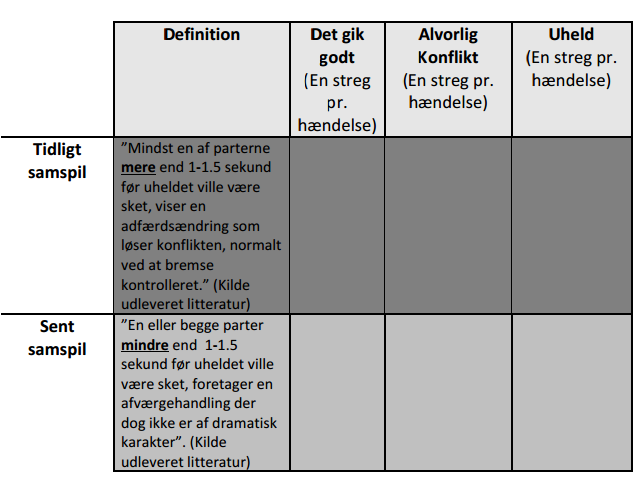
\includegraphics{figures/Billederogfigur/obstabel.png} %papir fra vejledern
 %\end{adjustbox}
  %\caption{Adfærdsregistreringstabel}
  %\label{fig:adfregtabel}
%\end{figure}
%\\\\
\textbf{"Det	gik	godt"} er defineret som en passering af konfliktpunktet, hvor situationen
har	været under kontrol og der har været afstand mellem parterne.8
%\\\\
\textbf{"Alvorlig konflikt"}	er defineret ud af en afværgehandling, som ville have ført til en kollision mellem to parter. Afværgehandlingen sker inden for 1-1.5 sekund før den mulige	kollision%(udleveret	litteratur).
%~\\\\
\textbf{"Uheld"} er defineret ved en kollision mellem to parter.
%~\\\\
Bemærk ved udførselen af denne metode blev der set bort fra isolerede ankomster, eftersom det ikke ville have haft indflydelse på vores konflikanalyse. Herefter blev målingerne fra TA-værdien brugt, hvilket kan ses på -cref{fig:maalingerfrabegge}, og alt andet ved observationen er det samme som det forrige %-cref{sub:dyb_undersoelse}
, hvor TA-værdien blev undersøgt.
%~\\\\
Det blev taget tid for hver reaktion for konflikt, således der kunne identificeres om der var sensamspil eller tidlig. Derudover blev der også set om konflikten gik godt eller om der var tale om alvorlig konflikt, som er defineret som sensamspil. De opnåede resultater kan ses på %-cref{fig:adfregtabelresult}.
Resultaterne fra TA-værdi og adfærdsregistering sættes sammen
\begin{figure}[htbp]
  \centering
  \begin{adjustbox}{max width=\textwidth}
    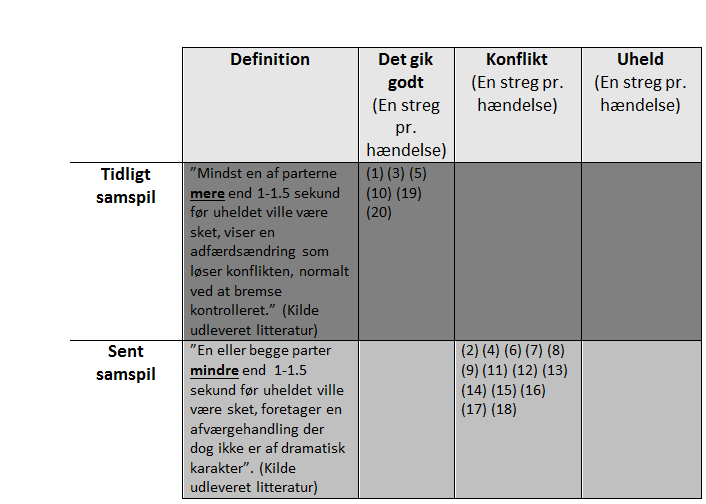
\includegraphics{figures/Billederogfigur/obstabelresult.png} %papir fra vejledern
 \end{adjustbox}
  \caption{Adfærdsregistreringstabel med resultater}
  \label{fig:adfregtabelresult}
\end{figure}
Der var en hypotese om, at hvis antallet af tidlige samspil stiger og antallet af sene samspil falder, så vil trafiksikkerheden fra området blive forøget. Ses der på adfærdsregisteringen -cref{fig:adfregtabelresult}, så kan der observeres, at der var flere sene samspil end tidlige samspil. Det vil ifølge vores hypotese pege på, at sikkerheden er dårlig ved netop dette sted. Ud fra TA-værdien kunne der også bekræftes, at sikkerheden ikke er helt optimalt.
Ud fra TA-grafen kan der ses, at 7 ud af 20 konflikter ikke er alvorlige, hvoraf 13 ud af 20 er alvorlige. Det svar til, at 65 procent af konflikterne er alvorlige, hvoraf resterne 35 procent er mindre alvorlige, og som ikke har en stor betydning for områdets sikkerhed.
